\section{Introduction}
	This paper introduces a method to be used for indoor painting detection. 
	
	
	\todo{What makes this work useful?}
	
	\todo{Why should someone spend time to read this paper}
	
	\todo{clarification of title and context}
	
	\todo{which problem has been solved}
	
	\todo{overview of related work}
	
	\todo{benefits and shortcomings of related work}
	
	\todo{overview of your own contributions}
	This paper contains $x$ contributions:
	\todo{overview of results}
	
	\todo{why these results are useful}
	
	\todo{overview of structure of the paper}
	In section 2 ...
	
	\subsection{Overview}
	The succeeding sections of this paper will discuss the implemntation of the proposed algorithm. Section \ref{sec:painting_detection} will discuss the inner workings of the algorithm. Section \ref{sec:evaluation_method} will describe the used performance metrics to evaluate the effectiveness of the algorithm. Section \ref{sec:results} will describe the expermintal results
	

	
	\begin{figure}
		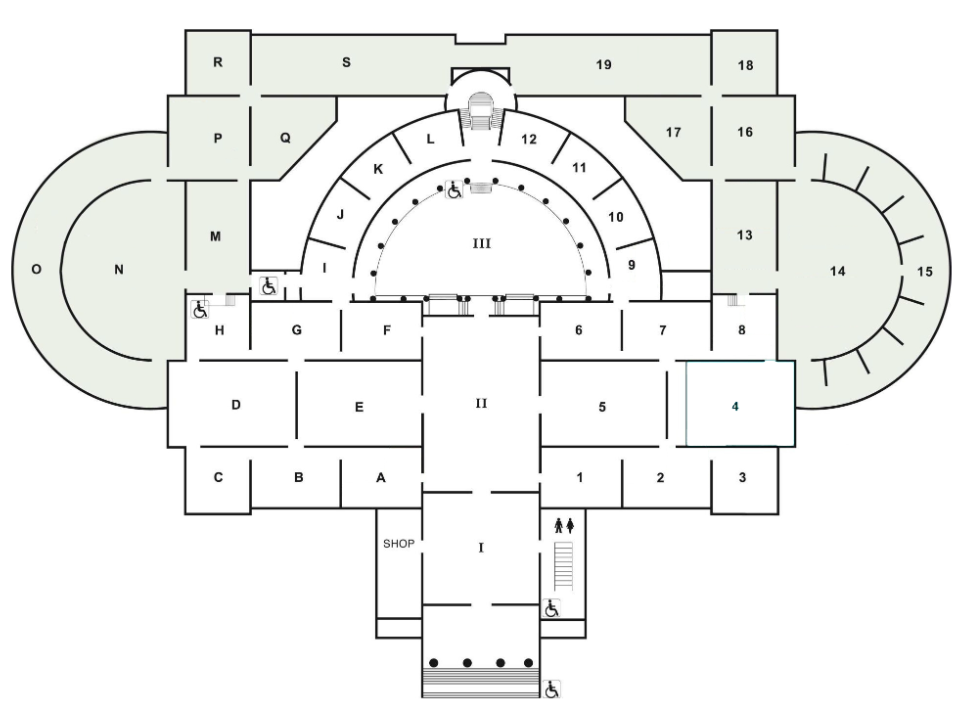
\includegraphics[width=\linewidth]{groundplan_msk}
		\caption{A ground plan of The Museum of Fine Arts, Ghent. }
		\label{fig:groundplan_msk}
	\end{figure}